\documentclass[margincite, leqno]{sl2art}

\usepackage{mathtools}

\usepackage{tikz}
\usepackage{todonotes}

%silence amsthm warning about \qedhere
\makeatletter
\def\qed@warning{}
\makeatother

\numberwithin{equation}{section}

\usepackage[export]{adjustbox}
\usepackage{graphicx,subcaption}
\graphicspath{{fig/}}

\usepackage{enumitem}

\newlist{thmenum}{enumerate}{1}
\setlist[thmenum]{label=(\alph*)}

\newcommand{\nr}{N}
\newcommand{\set}[1]{\left\{ \def\given{\ \middle| \ }  #1 \right\}  }
\newcommand{\defeq}{\mathrel{:=}}
\NewDocumentCommand{\iso}{}{\cong}
\DeclareMathOperator{\tr}{tr}
\DeclareMathOperator{\id}{id}
\DeclareMathOperator{\End}{End}
\renewcommand{\hom}{\operatorname{Hom}}

\NewDocumentCommand{\nset}{m}{\left[#1\right]}

\renewcommand{\Re}{\operatorname{Re}}
\renewcommand{\Im}{\operatorname{Im}}


\NewDocumentCommand{\dif}{}{\,\mathrm{d}}

\NewDocumentCommand{\bigoh}{}{\mathrm{O}}

\NewDocumentCommand{\du}{}{\amalg}

%use ifempty from xparse
\ExplSyntaxOn
\DeclareExpandableDocumentCommand{\IfEmptyTF}{mmm}
 {
    \tl_if_empty:nTF {#1} {#2} {#3}
 }
\ExplSyntaxOff

%fix spacing with paried delimiters
%use these for function arguments
\def\leftfun#1{\mathopen{}\left#1}
\def\rightfun#1{\right#1}

%useful for defining named functions
\NewDocumentCommand{\ParenIfNonempty}{m}{%
  \IfEmptyTF{#1}{%
  }{%
    \leftfun(#1\rightfun)%
  }
}

\NewDocumentCommand{\ii}{}{\mathsf{i}}
\NewDocumentCommand{\tu}{}{2 \pi \ii}

\NewDocumentCommand{\evec}{m}{\mathbf{e}_{#1}}

\NewDocumentCommand{\slg}{}{\operatorname{SL}_2(\mathbb{C})}
\NewDocumentCommand{\sla}{}{\mathfrak{sl}_2}
\NewDocumentCommand{\pslg}{}{\operatorname{PSL}_2(\mathbb{C})}
\NewDocumentCommand{\pjsp}{O{\mathbb{C}}}{\operatorname{#1 P}^{1}}
\DeclareMathOperator{\hyp}{hyp}
\NewDocumentCommand{\qn}{}{\triangleleft}
\NewDocumentCommand{\qninv}{}{\mathbin{\overline{\triangleleft}}}

\NewDocumentCommand{\qgrplong}{O{\xi}}{\mathcal{U}_{#1}(\mathfrak{sl}_2)}
\NewDocumentCommand{\qgrp}{O{\xi}}{\mathcal{U}_{#1}}
\NewDocumentCommand{\weyl}{O{\xi}}{\mathcal{W}_{#1}}

\NewDocumentCommand{\mer}{}{\mathbf{m}}
\NewDocumentCommand{\lon}{}{\mathbf{l}}
\NewDocumentCommand{\extr}{m}{M_{#1}}
\NewDocumentCommand{\comp}{m}{S^3 \setminus #1}
\DeclareMathOperator{\lk}{Lk}

\NewDocumentCommand{\homol}{m m}{\operatorname{H}_{#1}\leftfun(#2\rightfun)}
\NewDocumentCommand{\cohomol}{m m}{\operatorname{H}^{#1}\leftfun(#2\rightfun)}

%all Reidemeister moves in one macro
\ExplSyntaxOn
\NewDocumentCommand{\reid}{m O{}}{
  \bool_case:nTF
  {
    {\str_if_eq_p:NN {#1} {1} } { \operatorname{R}\sb{1} }
    {\str_if_eq_p:NN {#1} {1f} } { \operatorname{R}\sb{1}^{\operatorname{fr}} }
    {\str_if_eq_p:NN {#1} {2} } { \operatorname{R}\sb{2}^{#2} }
    {\str_if_eq_p:NN {#1} {2a} } { \operatorname{R}\sb{2}^{\operatorname{a}} }
    {\str_if_eq_p:NN {#1} {2b} } { \operatorname{R}\sb{2}^{\operatorname{b}} }
    {\str_if_eq_p:NN {#1} {3} } { \operatorname{R}\sb{3} }
  }
  { } %matches
  { } %unmatched
}
\ExplSyntaxOff

\NewDocumentCommand{\modcat}{m}{#1\operatorname{-mod}}
\NewDocumentCommand{\tsunit}{}{\mathbf{1}}

\NewDocumentCommand{\sclbrak}{m}{\left\langle #1 \right \rangle}

\NewDocumentCommand{\point}{}{\cdot}

\NewDocumentCommand{\repvar}{m}{\mathsf{R}\leftfun(#1\rightfun)}
\NewDocumentCommand{\admvar}{m}{\mathsf{A}\leftfun(#1\rightfun)}
\NewDocumentCommand{\logvar}{m}{\mathfrak{F}\leftfun(#1\rightfun)}
\NewDocumentCommand{\admvarbdry}{m}{\mathsf{A}^{\partial}_{#1}}

\NewDocumentCommand{\csbun}{O{}}{\mathcal{E}^{#1}}
\NewDocumentCommand{\qbun}{O{\nr} O{}}{\mathcal{E}_{#1}^{#2}}
\NewDocumentCommand{\qbunbig}{O{\nr} O{}}{\tilde{\mathcal{E}}_{#1}^{#2}}

\NewDocumentCommand{\qfunc}{O{\nr} m}{\mathcal{Z}_{#1}^{\psi}\ParenIfNonempty{#2}}

\NewDocumentCommand{\qinv}{O{\nr} m}{\mathrm{Z}_{#1}^{\psi}\ParenIfNonempty{#2}}

\NewDocumentCommand{\actq}{O{\nr} m m}{%
  \mathcal{S}_{#1}\leftfun(#2
  \IfEmptyTF{#3}{%
    \rightfun)
  }{%
    \middle|#3\rightfun)%
  }
}

\NewDocumentCommand{\act}{ m m}{%
  \mathcal{S}\leftfun(#1
  \IfEmptyTF{#2}{%
    \rightfun)
  }{%
    \middle|#2\rightfun)%
  }
}


\NewDocumentCommand{\stint}{O{\nr} m m}{%
  J_{#1}\leftfun(#2
  \IfEmptyTF{#3}{%
    \rightfun)
  }{%
    \middle|#3\rightfun)%
  }
}

\NewDocumentCommand{\stintadj}{O{\nr} m m}{%
  \widetilde{J}_{#1}\leftfun(#2
  \IfEmptyTF{#3}{%
    \rightfun)
  }{%
    \middle|#3\rightfun)%
  }
}

\NewDocumentCommand{\crossingfunction}{O{\nr} m m m}{
  \Omega_{#1}^{#2}\leftfun(#3
  \IfEmptyTF{#4}{%
    \rightfun)
  }{%
    \middle|#4\rightfun)%
  }
}

\NewDocumentCommand{\crossingfunctionclass}{m m}{
  \Omega^{#1}
  \IfEmptyTF{#2}{%
  }{%
    \leftfun(#2\rightfun)%
  }
}

\NewDocumentCommand{\lkfunc}{O{\nr} m}{\mathcal{L}_{#1}\ParenIfNonempty{#2}}
\NewDocumentCommand{\lklog}{O{} m}{\psi_{#1}\ParenIfNonempty{#2}}

\NewDocumentCommand{\qcat}{O{\nr}}{\mathsf{C}_{#1}}
\NewDocumentCommand{\tcat}{O{\nr}}{\mathsf{T}_{#1}}
\NewDocumentCommand{\vect}{}{\mathsf{Vect}}

\NewDocumentCommand{\shadset}{}{\mathsf{U}}

% (quantum) dilogs and q-series stuff
\NewDocumentCommand{\pf}{O{} m }{\varphi_{#1}\ParenIfNonempty{#2}}
\NewDocumentCommand{\pfl}{O{\nr} m}{\phi_{#1}\ParenIfNonempty{#2}}

\NewDocumentCommand{\qlfl}{O{\nr} m m}{%
  \lambda_{#1}\leftfun(#2
  \IfEmptyTF{#3}{%
    \rightfun)
  }{%
    \middle|#3\rightfun)%
  }
}

\NewDocumentCommand{\dll}{m }{\operatorname{L}\ParenIfNonempty{#1}}

\newcommand{\evup}[1]{\operatorname{ev}^\uparrow_{#1}}
\newcommand{\coevup}[1]{\operatorname{coev}^\uparrow_{#1}}
\newcommand{\evdown}[1]{\operatorname{ev}^\downarrow_{#1}}
\newcommand{\coevdown}[1]{\operatorname{coev}^\downarrow_{#1}}

\NewDocumentCommand{\lN}{}{\mathrm{N}}
\NewDocumentCommand{\lW}{}{\mathrm{W}}
\NewDocumentCommand{\lS}{}{\mathrm{S}}
\NewDocumentCommand{\lE}{}{\mathrm{E}}
\NewDocumentCommand{\up}{}{\uparrow}
\NewDocumentCommand{\dn}{}{\downarrow}

% macros borrowed from Colleen Delaney
\newcommand{\parcen}[1]{\phantom{(}#1\phantom{)}}
\newcommand{\br}{to [out=00,in=180]}


\declaretheorem[style=bigtheorem,title=Theorem,refname={Theorem,
Theorems}]{bigtheorem}
\declaretheorem[style=bigtheorem,title=Conjecture,refname={Conjecture,
Conjectures}]{conjecture}
\declaretheorem[style=theorem]{proposition}
\declaretheorem[style=theorem,sibling=proposition]{theorem}
\declaretheorem[style=theorem,sibling=proposition]{lemma}
\declaretheorem[style=theorem,sibling=proposition]{claim}
\declaretheorem[style=theorem,sibling=proposition]{corollary}
\declaretheorem[style=definition,sibling=proposition]{definition}
\declaretheorem[style=definition,sibling=proposition]{remark}
\declaretheorem[style=definition,sibling=proposition]{example}
\declaretheorem[style=definition,sibling=proposition]{Warning}

\declaretheorem[style=theorem, parent=]{step}

%\usepackage{showlabels}

\usepackage{cochineal}

\usepackage[noabbrev,capitalize]{cleveref}
\crefname{equation}{equation}{equations}
\Crefname{equation}{Equation}{Equations}
\crefname{bigtheorem}{Theorem}{Theorems}
\Crefname{bigtheorem}{Theorem}{Theorems}
\crefname{step}{Step}{Steps}
\Crefname{step}{Step}{Steps}
\crefname{conjecture}{Conjecture}{Conjectures}
\Crefname{conjecture}{Conjecture}{Conjectures}

\addbibresource{sources.bib}

\title{State integrals for the quantized \(\slg\) Chern-Simons invariant}
\author{Calvin McPhail-Snyder}
\address{Department of Mathematics, Duke University}
\email{calvin@sl2.site}

\begin{document}

\begin{abstract}
  Previous work of the author and N.\ Reshetikhin defines an
  invariant \(\operatorname{Z}_{N}^{\psi}(K, \rho, \mu)\) of a knot
  \(K\), a representation \(\rho \colon \pi_{1}(S^{3} \setminus K) \to
  \operatorname{SL}_{2}(\mathbb{C})\), and a logarithm \(\mu\) of a
  meridian eigenvalue of \(\rho\).
  It can be interpreted as a geometric twist of the Kashaev invariant
  or as a quantization of the \(\operatorname{SL}_{2}(\mathbb{C})\)
  Chern-Simons invariant and is defined via a discrete state-sum
  involving quantum dilogarithms.
  In this paper we show how to express
  \(\operatorname{Z}_{N}^{\psi}(K, \rho, \mu)\) as a sum over contour
  integrals in a space parametrizing hyperbolic structures on the
  knot complement.
  Such state integral presentations are an important step in
  determining the asymptotics of quantum invariants as predicted by
  the Volume Conjecture.
  We discuss this perspective and the remaining obstacles to
  establishing exponential growth of \(\operatorname{Z}_{N}^{\psi}\).
\end{abstract}

\subjclass{Primary 57K16, secondary 57K32, 58J28}
\keywords{complex Chern-Simons invariant, hyperbolic volume, quantum
hyperbolic invariants, quantum dilogarithm, volume conjecture, state integral}

\maketitle

%\tableofcontents
%\listoftodos

\section{Introduction}%
\label{sec:Introduction}

\subsection{Background and motivation}%
\label{sec:Background and motivation}

Kashaev's \defemph{Volume Conjecture} \cite{Kashaev1997} proposes a
striking connection between the geometry of hyperbolic knots and
their quantum invariants.
This conjecture appears to be related to quantum \(\slg\)
Chern-Simons theory, a TQFT arising as a complexification
\cite{Gukov2005} or analytic continuation \cite{Witten2010} of the
more familiar quantum \(\operatorname{SU}(2)\) Chern-Simons theory
\cite{zbMATH04092352}.
A number of authors
\cite{Baseilhac2004,Bonahon2021,Kashaev2005,McPhailSnyderVolume} have
constructed geometric quantum invariants that can be interpreted as
candidates for a mathematical realization of \(\slg\) Chern-Simons theory.

We discuss some typical features of a candidate mathematical realization.%
\note{
  In the terminology of \cref{sec:negative type} these are cyclic
  type invariants.
  There are also related but inequivalent principal type invariants.
}
For concreteness let \(K\) be a hyperbolic knot in \(S^{3}\),
although some versions are additionally or instead defined for closed
\(3\)-manifolds or related objects.
A realization is a family of functions
\[
  \mathcal{Z}_{\nr} \colon \mathsf{X}(K) \to \mathbb{C}
\]
for \(\nr\) a positive integer related to the level and
\(\mathsf{X}(K)\) a space parametrizing hyperbolic structures on
\(\comp{K}\); it is usually a version of the \(\slg\) character
variety of \(\comp{K}\).
Let \(\varsigma_{K} \in \mathbb{C}/ 2 \pi \ii \mathbb{Z}\) be the
\(\slg\) Chern-Simons invariant of the canonical structure
\(\rho_{\hyp}\) of \(K\), normalized so \(2 \pi \Re \varsigma_{K}\)
is the hyperbolic volume of \(K\).
A volume conjecture is the statement that (up to normalization and
some other details)
\begin{equation}
  \label{eq:asymptotics sign positive}
  \lim_{\nr \to \infty}
  \frac{
    \log \mathcal{Z}_{\nr}(K, \rho)
  }{
    \nr
  }
  =
  \varsigma_{K}
\end{equation}
for some \(\rho \in \mathsf{X}(K)\) that is not necessarily \(\rho_{\hyp}\).
We think of \(\nr \to \infty\) as the semiclassical limit.
The surprising observation is that this holds for \(\rho\) other than
\(\rho_{\hyp}\); Kashaev's original conjecture \cite{Kashaev1997} is
that it happens for the trivial hyperbolic structure \(1\).
In this case \(\mathcal{Z}_{\nr}(K,1)\) can be identified with a
value of the \(\nr\)th colored Jones polynomial of \(K\) \cite{Murakami2001}.
There is a standard ansatz (successful in some special cases) for
proving these conjectures that uses two steps.

\begin{step}[Establish integrals]
  \label{step 1}
  Show that the invariant is equivalent (perhaps asymptotically) to a
  \defemph{state integral}, a contour integral
  \[
    \mathcal{Z}_{\nr}(K, \rho) \sim
    \int_{\Gamma} e^{\nr \mathcal{S}(\mathbf{t})} \dif \mathbf{t}
  \]
  where \(\mathcal{S}\) is a holomorphic function that can be
  identified with the Chern-Simons functional.
  Sometimes instead one must consider a sum of such integrals.
\end{step}

In more detail, given a combinatorial description \(\mathcal{T}\) of
\(\comp{K}\) the domain of \(\mathcal{S}\) is a space
\(\Omega_{\mathcal{T}}\) parametrizing hyperbolic structures on the
individual pieces of \(\mathcal{T}\).
Critical points of \(\mathcal{S}\) are choices that combine together
to give a coherent structure on all of \(\comp{K}\) and the critical
value is the \(\slg\) Chern-Simons invariant.
For example, if \(\mathcal{T}\) is an ideal triangulation then
\(\Omega_{\mathcal{T}}\) parametrizes shapes of the tetrahedra and
critical points of \(\mathcal{S}\) are solutions of Thurston's gluing equations.

\begin{step}[Move the contour]
  \label{step 2}
  Show that
  \[
    \int_{\Gamma} e^{\nr \mathcal{S}(\mathbf{t})} \dif \mathbf{t}
    \sim
    \int_{\Gamma'} e^{\nr \mathcal{S}(\mathbf{t})} \dif \mathbf{t}
  \]
  where \(\Gamma'\) is a contour in saddle point position for a
  critical point corresponding to \(\rho_{\hyp}\).
\end{step}

The maximum critical value of \(\Re \mathcal{S}\) is \(\Re \varsigma_{K}\).
It occurs at a saddle point of \(\Re \mathcal{S}\) because
\(\mathcal{S}\) is a holomorphic function.
If \(\Gamma'\) is a contour passing through this saddle point in the
right way a standard \defemph{saddle-point approximation} by a
Gaussian integral gives the desired asymptotics \eqref{eq:asymptotics
sign positive}.

In general both steps require hard computations; a detailed
discussion of the analytic issues is given by
\citeauthor{zbMATH06684922} \cite{zbMATH06684922}.
\cref{step 1} requires re-writing a discrete sum as a (sum of)
integrals, typically by using the Poisson summation formula.
Ensuring that this is valid requires careful estimates on the size of
\(\mathcal{S}\) and related functions.

Previous work of the author \cite{McPhailSnyderVolume} uses the
holonomy \(R\)-matrices defined in joint work with N.\ Reshetikhin
\cite{McPhailSnyderAlgebra} to define a candidate mathematical
realization \(\qinv{}\) of complex Chern-Simons theory as described above.
In this paper we show that \(\qinv{}\) is equal to a sum of state integrals.
Our method does not require checking any inequalities and works for
any representation satisfying a natural, algebraic nondegeneracy condition.
To my knowledge this is the first example of an exact (not
asymptotic) state integral presentation of a cyclic type invariant.
Such integral presentations automatically occur for principal type
invariants, an inequivalent but related mathematical realization of
complex Chern-Simons theory (\cref{sec:negative type}).
Our results may clarify the relationship between these two branches.

\subsection{Our results}%
\label{sec:Our results}

Let \(K\) be an oriented, framed knot in \(S^{3}\) and \(\rho\)  a
decorated representation of \(K\), which is a representation \(\rho \colon
\pi_{1}(\comp{K}) \to \slg\) along with a choice of eigenspace for
the image of the peripheral subgroup under \(\rho\).
In particular this choice distinguishes an eigenvalue \(m\) of the
meridians of \(K\).
A \defemph{log-meridian} is a complex number \(\mu\) with \(e^{\tu \mu} = m\).
The main result of \cite{McPhailSnyderVolume} is the definition of a
sequence of invariants%
\note{
  In \cite{McPhailSnyderVolume} we wrote \(\qinv{}\) as depending on
  a \defemph{log-decoration} \(\mathfrak{s}\), which also includes a
  choice of log-longitude \(\lambda\).
  The normalization \(\qinv{}\) used here is independent of
  \(\lambda\) so we drop it from the notation.
}
\[
  \qinv{K, \rho, \mu} \in \mathbb{C}
\]
for integers  \(\nr \ge 2\).
We can view them as a quantization of the  \(\slg\) Chern-Simons
invariant, as a geometric twist of the Kashaev \cite{Kashaev1995} and
ADO \cite{Akutsu1992} invariants, or as a candidate mathematical
realization of \(\slg\) Chern-Simons theory.
The construction makes sense (and our results do too) for links and
tangles as well but for simplicity we restrict to the case of knots.

Let \(D\) be an open knot diagram of \(K\) (i.e\@ a \(1\)-\(1\)
tangle diagram whose closure is \(K\)).
Let \(E\) be the set of internal segments (edges) of \(D\).
Using quantum dilogarithms we define an \defemph{action} \(\actq{D,
\mu}{} \colon \mathbb{C}^{E} \to \mathbb{C}\) so that
\[
  t \mapsto e^{ \nr \actq{D, \mu}{t} } \colon  \mathbb{C}^{E} \to \mathbb{C}
\]
is a meromorphic function.
Given the choice of some additional gauge data \(u\) called a
\defemph{shadow coloring} the invariant of \cite{McPhailSnyderVolume}
is by definition a state sum
\[
  \qinv{K, \rho, \mu}
  =
  \frac{1}{\nr^{\operatorname{cr}(D)}}
  \sum_{n \in \nset{\nr}^{E}}
  e^{ \nr  \actq{D, \mu}{(\beta + n)/\nr} }
\]
where \(\nset{\nr} = \set{0, 1, \dots, \nr - 1}\) and
\(\operatorname{cr}(D)\) is the crossing number of \(D\).
The vector \(\beta \in \mathbb{C}^{E}\) encodes \((\rho, u)\).
For a vector \(k \in \mathbb{Z}^{E}\) with integer entries%
\note{%
  As discussed in \cref{rem:flattening vector} the choice of
  \(\mathbf{k}\) (along with \(\beta\)) determines a flattening
  of the octahedral decomposition associated to \(D\).
}
a \defemph{state integral} is
\begin{equation}
  \label{eq:state integral intro}
  \stint{D, \mu, \beta}{k}
  \defeq
  \int_{[0,1]^{E}}
  \exp \leftfun[ \nr ( \actq{D, \mu}{\beta/\nr + t} - \tu k \cdot t )
  \rightfun]
  \dif t
\end{equation}
In \cref{sec:State integrals big} we prove (\cref{main result}) that
\(\qinv{}\) is given by the sum over all state integrals:
\begin{equation}
  \label{eq:state integral sum intro}
  \qinv{K, \rho, \mu}
  =
  \nr^{(|E| - 1)/2}
  \sum_{k \in \mathbb{Z}^{E}}
  \stint{D, \mu, \beta}{k}
\end{equation}
The main technical difficulty is ensuring the contour of integration
avoids the poles of \(e^{\nr\actq{D, \mu}{}}\).
We discuss the required algebraic condition in \cref{sec:Gauge
transformations and admissibility}.
Once this is handled using the methods of
\cite{McphailSnyder2024octahedralcoordinateswirtingerpresentation}
re-writing the sum in terms of the integrals is an elementary
application of Fourier series.
In particular the convergence of the infinite sum is automatic.

As \(\nr \to \infty\) the functions \(\actq{D , \mu}{}\) to a
function \(\act{D}{}\) that we interpret as the Chern-Simons action.
In the literature \(\act{D}{}\) is frequently called the
\defemph{(Yokota) potential function} \cite{arXiv:math/0009165} and
denoted \(V\).
The critical points of \(\actq{D}{}\) are boundary-parabolic
representations of \(K\) and the critical values are their
Chern-Simons invariants.
As such \cref{main result} accomplishes \cref{step 1} towards proving
a volume conjecture for \(\qinv{}\).
We state this precisely, explain how the sum over \(\mathbb{Z}^{E}\)
is natural, and discuss barriers to \cref{step 2} in
\cref{sec:Formal asymptotics}.

\subsection{Cyclic and principal type invariants}
\label{sec:negative type}

There appear to be two inequivalent (but perhaps both natural)
branches of complex Chern-Simons theory.
Above we described \defemph{cyclic type} invariants
\cite{Baseilhac2004,Bonahon2021,Kashaev2005,McPhailSnyderVolume} that
\begin{itemize}
  \item are defined as a sum over a finite state space,
  \item are conjectured to exponentially grow as \(\nr \to \infty\), and
  \item are well-defined for any (or any geometrically
    non-degenerate) hyperbolic structure.
\end{itemize}
In contrast, \defemph{principal type} invariants
\cite{zbMATH06324352,arXiv:1305.4291,arXiv:2508.05120}
\begin{itemize}
  \item are defined using integrals over a noncompact, continuous state space,
  \item are conjectured to \emph{decay} as \(\nr \to \infty\), but
  \item are only defined when the hyperbolic structure satisfies a
    positivity condition so that the integrals converge.
\end{itemize}
These two branches are related to different quantizations of the moduli space of
\(\slg\) local systems.
Principal type invariants are related to the representations of
quantum cluster varieties defined by \citeauthor{zbMATH01607168}
\cite{zbMATH01607168} and \citeauthor{zbMATH05530519}
\cite{zbMATH05530519}.
These are infinite-dimensional representations analogous to the
principal series representations of \(\operatorname{SL}_{2}\).
The cyclic quantizations studied in detail by
\citeauthor{arXiv:2501.02316} \cite{arXiv:2501.02316} are
finite-dimensional and analogous to highest-weight modules.
Cyclic type invariants are more directly related to the Kashaev
invariant and the original Volume Conjecture.
It is typically easier to prove volume conjectures for principal type
invariants:
they are \emph{defined} in terms of integrals, so \cref{step 1} holds
automatically, subject to the positivity condition.

Asymptotic growth of cyclic type invariants has been established
only for knots with up to \(7\) crossings \cite{zbMATH06684922,
Ohtsuki2017, Ohtsuki2018} and for twist knots \cite{Chen2023II}.
For principal type invariants much more is known:
the invariant of \textcite{arXiv:2508.05120} satisfies the conjecture
for every hyperbolic manifold with totally geodesic boundary,
and the Andersen-Kashaev Teichm{\"u}ller TQFT satisfies it for twist
knots \cite{zbMATH07761477} and many other manifolds
\cite{arXiv:2410.10776, arXiv:2512.17437, arXiv:2512.23198}.
We hope that our result leads to a proof of asymptotic growth of
\(\qinv{}\) using similar techniques.

In addition, our work may lead to a better understanding of the
relationship between cyclic and principal invariants.
\textcite{arXiv:1305.4291} showed that their principal type TQFT can
be defined using integrals over compact state spaces.
This form of the partition function formally resembles the sum of
state integrals \eqref{eq:state integral sum intro} after a Wick
rotation and changing the overall sign of the action.
Their reformulation is accomplished via a Weil-Gel'fand-Zak transform
taking values in a space of quasi-periodic functions.
Similar quasi-periodic functions are used in the definition of
\(\qinv{}\) \cite{McPhailSnyderVolume} and this may lead to a more
precise relationship between the two constructions.

\subsection*{Acknowledgements}
I would like to thank Francis Bonahon, Effie Kalfagianni, Lillian
Pierce, and Ka Ho Wong for helpful conversations.

\section{Preliminaries}%
\label{sec:Preliminaries}

Here we give some preliminary facts about \(\slg\) representations of
link complements and octahedral decompositions.
For details see
\cite{McphailSnyder2022hyperbolicstructureslinkcomplements} and
\cite{McphailSnyder2024octahedralcoordinateswirtingerpresentation}.
\subsection{Diagrams and colorings}%
\label{sub:Diagrams}

\begin{definition}
  A \defemph{decorated representation} of a knot \(K\) is a
  representation \(\rho \colon \pi_{1}(\comp{K}) \to \slg\) and a choice
  of eigenspace for the image of each peripheral subgroup of \(K\)
  under \(\rho\).
\end{definition}

More formally, given a choice of peripheral subgroup \(\Pi \subset
\pi_{1}(\comp{K})\) a decoration is an eigenspace \(L \subset
\mathbb{C}^{2}\) of \(\rho(\Pi)\), which we take to be a right eigenspace.
This does not depend on the choice of peripheral subgroup: any other
choice is a conjugate \(y^{-1} \Pi y\) and the corresponding
eigenspace is \(L \rho(y)\).
An orientation of \(K\) determines a meridian \(\mer \in \Pi\) and
the decoration \(L\) determines an eigenvalue \(m \in \mathbb{C}^{\times}\) by
\[
  v \rho(\mer) = m^{-1} v
\]
where \(v\) is any nonzero element of \(L\).
The inverse is unfortunate but correct and is chosen to match the
conventions of \cite{McPhailSnyderAlgebra,McPhailSnyderVolume}.
Clearly \(m\) does not depend on the choice of \(\Pi\).

\begin{definition}
  Let \(K\) be an oriented, framed knot in \(S^{3}\).
  An \defemph{open diagram} of \(K\) is an oriented,
  blackboard-framed tangle diagram \(D\) with one incoming and one
  outgoing boundary component whose closure is a diagram of \(K\).
  The \defemph{segments} of \(D\) are the edges of its underlying graph.
  We call the two segments incident to the boundary of the tangle the
  \defemph{boundary segments}, call the remainder the
  \defemph{internal segments}, and write \(E\) for the set of
  internal segments of \(D\).
  Writing \(\operatorname{cr}(D)\) for the crossing number of the
  diagram we have \(2 \operatorname{cr}(D) = |E| + 1\).
\end{definition}

\begin{definition}
  A \defemph{decorated matrix} is a pair \((g, [v]) \in \slg \times
  \pjsp\) of a matrix \(g\) and a right eigenspace \([v]\) for \(g\).
  The \defemph{distinguished eigenvalue} of \((g, [v])\) is the \(m
  \in \mathbb{C}^{\times}\) satisfying
  \[
    vg = m^{-1} v.
  \]
  We define a binary operation on decorated matrices by
  \begin{equation}
    (g, [v]) \qn (h, [w])
    \defeq
    (h^{-1} g h, [v h])
  \end{equation}
  A \defemph{decorated \(\slg\)-coloring} of a tangle diagram \(D\)
  assigns decorated matrices to every arc of \(D\) subject to the
  crossing relations
  \begin{equation}
    \begin{aligned}
      &
      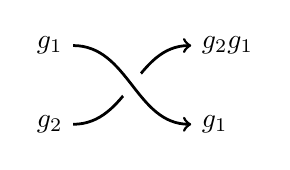
\begin{tikzpicture}[line width=1, baseline=30, scale=1]
        \draw[->] (0,0) node[left] {\(g_{2}\)} \br (1.5,1)
        node[right] {\(g_{2} \qn g_{1}\)};
        \draw[white, line width=10] (0,1) node[left] {} \br (1.5,0)
        node[right] {};
        \draw[->] (0,1) node[left] {\(g_{1}\)} \br (1.5,0)
        node[right] {\(g_{1}\)};
      \end{tikzpicture}
      &
      &
      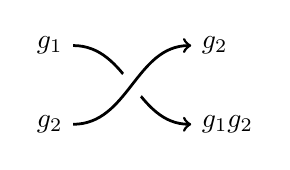
\begin{tikzpicture}[line width=1, baseline=30, scale=1]
        \draw[->] (0,1) node[left] {\(g_{1}\)} \br (1.5,0)
        node[right] {\(g_{1} \qninv g_{2}\)};
        \draw[white, line width=10] (0,0) node[left] {} \br (1.5,1)
        node[right] {};
        \draw[->] (0,0) node[left] {\(g_{2}\)} \br (1.5,1)
        node[right] {\(g_{2}\)};
      \end{tikzpicture}
    \end{aligned}
  \end{equation}
  where \(\qninv\) is the inverse of \(\qn\) defined by
  \(
    (g, [v]) \qninv (h, [w])
    \defeq
    (h g h^{-1}, [v h^{-1}]).
  \)
  We always require that a \(\slg\)-coloring of an open diagram
  assigns the same decorated matrix to both boundary segments, or
  equivalently that it gives a well-defined coloring of the closure.
\end{definition}

The Wirtinger presentation of \(\pi_{1}(\comp{K})\) makes it clear
that decorated representations of \(K\) are in bijection with
decorated \(\slg\)-colorings of \(D\) so we denote both by \(\rho\).
To define our invariant we need to make an additional choice of
diagram-dependent gauge data.%
\note{
  Our invariant is defined in terms of the octahedral decomposition
  associated to \(D\).
  This is a semi-ideal triangulation with two non-ideal vertices.
  The extra degrees of freedom are related to the choice of location
  of these vertices.
}
The value of \(\qinv{}\) is independent of this choice.

\begin{definition}
  A \defemph{shadow coloring} \((\rho, u)\) of a diagram \(D\) is a
  decorated \(\slg\)-coloring \(\rho\) of \(D\) along with an
  assignment \(u \colon j \mapsto u_{j}\) of column vectors \(u_{j} \in
  \mathbb{C}^{2}\) to the regions \(j\) of \(D\), subject to the rule
  \begin{equation}
    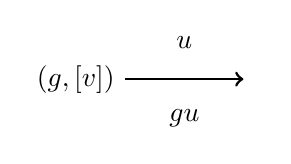
\begin{tikzpicture}[line width=1, baseline=00, scale=1]
      \draw[->] (0,0) node[left] {\((g, [v])\)} to (1.5,0) node[right] {};
      \node[above] at (.75,0.25){\(u\)};
      \node[below] at (.75,-0.25){\(g u\)};
    \end{tikzpicture}
  \end{equation}
  In the diagram above we say the region labeled by \(u\) is
  \defemph{above} the segment.
\end{definition}

It is not hard to see that a shadow coloring is determined uniquely
by the vector \(u_{0} \in \mathbb{C}^{2}\) assigned to the topmost
region of \(D\) (or to any other region).

\begin{definition}
  A shadow coloring of a diagram \(D\) defines \defemph{region parameters}
  \begin{equation}
    a_{j} \defeq \evec{1} u_{j}
    \text{ for each region \(j\)}
  \end{equation}
  and \defemph{segment parameters}
  \begin{equation}
    b_{i} \defeq
    -
    \frac{
      v_{i} \evec{2}
    }{
      v_{i} u_{i^{\uparrow}}
    }
    \text{ for each segment \(i\)}
  \end{equation}
  where \(i^{\up}\) is the region above segment \(i\):
  \[
    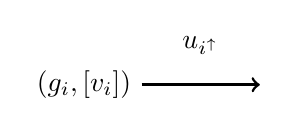
\begin{tikzpicture}[line width=1, baseline=00, scale=1]
      \draw[->] (0,0) node[left] {\((g_{i}, [v_{i}])\)} to (1.5,0)
      node[right] {};
      \node[above] at (.75,0.25){\(u_{i^{\uparrow}}\)};
    \end{tikzpicture}
  \]
  If none of the region or segment parameters are \(0\) or \(\infty\)
  we say the shadow coloring is \defemph{admissible}.
\end{definition}

\begin{definition}
  A shadow coloring \((\rho, u)\) of an open diagram \(D\) is
  \defemph{normalized} if it is admissible and the segment parameter
  assigned to the open segments is \(1\).
\end{definition}

Clearly one can always choose a normalized coloring by rescaling the
vectors \(u_{i}\).
This is a special case of the type (B) gauge transformation defined below.

\subsection{Gauge transformations and nondegeneracy }%
\label{sec:Gauge transformations and admissibility}

The diagram \(D\) determines a semi-ideal triangulation
\(\mathcal{T}_{D}\) of \(\comp{K}\) (with two non-ideal points)
called the \defemph{octahedral decomposition};
we refer to \cite{Kim2018} for a detailed discussion and
\cite{McphailSnyder2022hyperbolicstructureslinkcomplements,
McphailSnyder2024octahedralcoordinateswirtingerpresentation} for the
relationship to our parameters.
\(\mathcal{T}_{D}\) assigns each crossing of \(D\) four tetrahedra,
with one in each corner of the crossing.
The segment parameters naturally parametrize hyperbolic structures on
these tetrahedra in terms of \defemph{shape parameters} \(z_{k}\).
Labeling the segments and corners of a crossing as
\begin{equation}
  \label{eq:crossing labeled}
  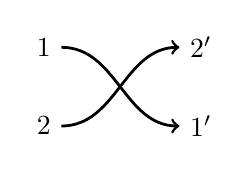
\begin{tikzpicture}[line width=1, baseline=30, scale=1]
    \draw[->] (0,0) node[left] {\({2}\)} \br (1.5,1) node[right] {\({2'}\)};
    %    \draw[white, line width=10] (0,1) node[left] {} \br (1.5,0)
    % node[right] {};
    \draw[->] (0,1) node[left] {\({1}\)} \br (1.5,0) node[right] {\({1'}\)};
    \draw (0.75,1) node {\(\lN\)};
    \draw (0,0.5) node {\(\lW\)};
    \draw (0.75,0) node {\(\lS\)};
    \draw (1.5,0.5) node {\(\lE\)};
  \end{tikzpicture}
\end{equation}
the shape parameters of the tetrahedra are given by
\begin{equation}
  \label{eq:shape parameters}
  \begin{aligned}
    z_{\operatorname{N}} &= \left( \frac{b_{2'}}{b_{1}} \right)^{\epsilon}
    &
    z_{\operatorname{S}} &= \left( \frac{b_{2}}{b_{1'}}\right)^{\epsilon}
    \\
    z_{\operatorname{W}} &= \left(\frac{b_{2}}{m b_{1}}\right)^{\epsilon}
    &
    z_{\operatorname{E}} &= \left(\frac{m b_{2'}}{b_{1'}}\right)^{\epsilon}
  \end{aligned}
\end{equation}
where \(\epsilon\) is the sign of the crossing.
The shape parameters arise as cross ratios of the positions of the
vertices in \(\pjsp\).
In particular a tetrahedron is geometrically degenerate when its
shape parameter lies in \(\set{0, 1, \infty}\).

If a shadow coloring is admissible as defined above then none of the
shape parameters of \(\mathcal{T}_{D}\) are \(0\) or \(\infty\).%
\note{
  Strictly speaking a shape parameter \(z = z^{0}\) corresponds to a
  pair of edges of a vertex-ordered tetrahedron, with the other edge
  pairs assigned \(z^{1} = 1/(1 - z^{0})\) and \(z^{2} = 1 - 1/z^{0}\).
  Admissibility means that a particular preferred edge pair is not
  \(0\) or \(\infty\).
}
This is a necessary condition to define \(\qinv{}\), and every
representation \(\rho\) is gauge-equivalent to an admissible one.
Since \(\qinv{}\) is gauge-invariant this allows us to define it for
any \(\rho\).

\begin{definition}[\protect{\cite[Section
  4]{McphailSnyder2024octahedralcoordinateswirtingerpresentation}}]
  \label{def:gauge transformation}
  Let \((\rho, u)\) be a shadow coloring of \(D\) with segment colors
  \(i \mapsto (g_{i}, [v_{i}])\) and region colors \(j \mapsto u_{j}\).
  A \defemph{gauge transformation} of it is a coloring of the form
  \begin{itemize}
    \item[(A)] \(i \mapsto (h^{-1} g_i h, L_i h)\) and \(j \mapsto h^{-1} u_j\)
    \item[(B)] \(i \mapsto (g_i, L_i)\) and \(j \mapsto h^{-1} u_j\)
  \end{itemize}
  for some \(h \in \slg\).
  We say the new colorings are the images of \defemph{type (A)} and
  \defemph{type (B)} gauge transformations  \defemph{by \(h\)}.
\end{definition}

\begin{lemma}[\protect{\cite[Theorem
  2]{McphailSnyder2024octahedralcoordinateswirtingerpresentation}}]
  Let \(\rho\) be a decorated representation and \(D\) an open diagram of \(K\).
  Any shadow coloring \((\rho, u)\) of \(D\) is gauge-equivalent to
  one with an admissible shadow coloring.
\end{lemma}

While we can ensure the shape parameters lie in \(\mathbb{C}\setminus
\set{0}\) we cannot necessarily ensure they avoid \(1\).
Having shape parameter \(1\) is independent of the choice of shadow
coloring and is equivalent to a natural condition on the decorated
representation:

\begin{definition}
  A crossing with a decorated \(\slg\)-coloring
  \[
    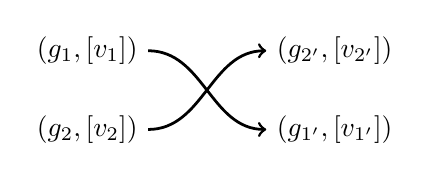
\begin{tikzpicture}[line width=1, baseline=30, scale=1]
      \draw[->] (0,0) node[left] {\((g_{2}, [v_{2}])\)} \br (1.5,1)
      node[right] {\((g_{2'}, [v_{2'}])\)};
      %    \draw[white, line width=10] (0,1) node[left] {} \br
      % (1.5,0) node[right] {};
      \draw[->] (0,1) node[left] {\((g_{1}, [v_{1}])\)} \br (1.5,0)
      node[right] {\((g_{1'}, [v_{1'}])\)};
    \end{tikzpicture}
  \]
  is \defemph{pinched} if \([v_{1}] = [v_{2}]\), equivalently
  \([v_{i}] = [v_{j}]\) for any pair \((i,j)\) of adjacent segments.
  (Note that this condition does not depend on a choice of shadow coloring.)
  A coloring of a diagram is pinched if any of its crossings are.
  If \(\rho\) is a decorated representation of \(K\) and \(D\) an
  open diagram of \(K\) we say \(D\) is  \defemph{\(\rho\)-pinched}
  if the coloring induced by \(\rho\) is pinched (and conversely that
  \(\rho\) is  \defemph{\(D\)-pinched}).
  If no crossing is pinched we say \((D, \rho)\) is \defemph{smooth}.
\end{definition}

A nugatory crossing is always pinched.
If \(D\) is a crossing-minimal diagram it has no nugatory crossings
and in this case most (but not all) nontrivial representations
\(\rho\) are \(D\)-smooth.
For example, up to gauge transformation the \(8_{5}\) knot has \(11\)
boundary-parabolic representations \cite{Kim2018}.
In the standard diagram \(D\) \cite[Figure 28]{Kim2018} of this knot
\(10\) are smooth and \(1\) is pinched.
\(8_{5}\) is hyperbolic and its discrete faithful representation is
\(D\)-smooth.
According to the database of boundary-parabolic representations computed by
\citeauthor{DiagramSite} \cite{DiagramSite} this pattern holds in general:
for crossing-minimal \(D\) most but not all representations are
\(D\)-smooth, but the hyperbolic holonomy representation is always smooth.

In the standard terminology a not \(\rho_{\hyp}\)-pinched diagram is
said to be \defemph{essential}.%
\note{
  More formally the associated octahedral decomposition is essential.
}
By \cite[Theorem
3]{McphailSnyder2024octahedralcoordinateswirtingerpresentation} being
essential is equivalent to a purely group-theoretic condition called
\defemph{arc-faithfulness}.
It is not hard to see that if \(D\) is not arc-faithful then it is
pinched for every decorated representation \(\rho\).
It is natural to conjecture (see \cite[Section
5]{McphailSnyder2024octahedralcoordinateswirtingerpresentation}) that
any hyperbolic knot has an arc-faithful diagram.
It is known that any reduced alternating diagram of a hyperbolic knot
is arc-faithful.

At any pinched crossing the shape parameters are \(1\) so the
\(R\)-matrix elements defining \(\qinv{}\) encounter the poles and
zeros of the quantum dilogarithm.
One can show that these cancel, but in a delicate way that prevents
our state integrals from being well-defined.
More generally to avoid the singularities we need to ensure that no
shape parameter has norm \(1\), and if no crossings are pinched then
we can achieve this via a gauge transformation.

\begin{lemma}[\protect{\cite[Corollary
  5.3]{McphailSnyder2024octahedralcoordinateswirtingerpresentation}}]
  \label{thm:avoid unit circle}
  Let \(\rho\) be a decorated representation of a knot \(K\) and
  \(D\) be an open diagram of \(K\).
  Suppose that \(D\) is not \(\rho\)-pinched.
  Then there is a representation \(\rho'\) gauge-equivalent to
  \(\rho\) and a shadow coloring \((\rho', u)\) of \(D\) in which  no
  shape parameter has norm \(1\).
  In this case we say \((\rho', u)\) \defemph{avoids the unit circle}.
\end{lemma}

\subsection{Segment equations}%
\label{sec:Segment equations}

The segment parameters have a natural geometric
interpretation: they parametrize the locations of the ideal vertices
of the octahedral decomposition.
Following
\cite{McphailSnyder2024octahedralcoordinateswirtingerpresentation} we
obtained the segment parameters from a shadow coloring
but one can also work in the opposite direction.
An assignment of numbers \(b_{i}\) to the segments of \(D\) induces a
decorated representation of \(K\) if and only if the shape parameters
satisfy Thurston's gluing equations.
These can be summarized in one equation for each segment.

\begin{definition}
  \label{def:segment equations}
  Choose a meridian eigenvalue \(m \in \mathbb{C} \setminus \set{0}\).
  Assign a variable \(b_{i} \in \mathbb{C} \setminus \set{0}\) to
  every segment of a cut presentation \(D\) (with the variables of
  the boundary segments matching as usual).
  Use these to assign each corner of the diagram a shape parameter
  \(z_{k}\) as in \cref{eq:shape parameters}; we assume that the
  \(b_{i}\) are chosen so that no \(z_{k}\) is \(1\).
  Labeling a crossing of sign \(\epsilon\) as in \eqref{eq:crossing
  labeled} the choice of \(m\) and \(b_{i}\) determine parameters
  \(a_{i}\) for each segment%
  \note{
    We denote these by \(a_{i}\) because they correspond to ratios of
    the region parameters \(a_{j}\).
  }
  by
  \begin{equation}
    \label{eq:segment a vars}
    \begin{aligned}
      a_{1}
      &=
      m^{\epsilon}
      \frac{
        1 - z_{\lW}
      }{
        1 - z_{\lN}
      }
      &
      a_{4}
      &=
      m^{-\epsilon}
      \frac{
        1 - z_{\lE}
      }{
        1 - z_{\lN}
      }
      \\
      a_{2}
      &=
      m^{-\epsilon}
      \frac{
        1 - z_{\lS}
      }{
        1 - z_{\lW}
      }
      &
      a_{3}
      &=
      m^{\epsilon}
      \frac{
        1 - z_{\lS}
      }{
        1 - z_{\lE}
      }
    \end{aligned}
  \end{equation}
  The construction above assigns every segment \emph{two} parameters
  \(a_{i}\) and \(a_{i}'\) from the crossings at both ends.
  The \defemph{segment equations} say that these parameters agree for
  each segment.
\end{definition}

The segment equations were first studied by
\textcite{arXiv:math/0009165} and are discussed in detail by \textcite{Kim2018}.
Our formulation follows the conventions of
\cite{McphailSnyder2022hyperbolicstructureslinkcomplements,McphailSnyder2024octahedralcoordinateswirtingerpresentation}.

\begin{proposition}
  \label{thm:segment solutions are reps}
  For an open knot diagram \(D\) there is a bijection between the sets of
  \begin{thmenum}
  \item solutions of the segment equations of \(D\) with meridian
    eigenvalue \(m\)
  \item shadow-colored decorated representations \((\rho, u)\) with
    meridian eigenvalue \(m\) that are not \(D\)-pinched
    \qedhere
  \end{thmenum}
\end{proposition}

\begin{proof}
  Suppose we have a solution of the segment equations with meridian
  eigenvalue \(m\).
  Then by definition there is a well-defined assignment of parameters
  \(a_{i}\) to the segments of \(D\) that give a non-pinched
  \defemph{octahedral coloring} of \(D\) in the sense of
  \cite{McphailSnyder2022hyperbolicstructureslinkcomplements}.
  Call the set of such colorings \(Y\).
  A point of \(Y\) gives a solution of the segment equations (by
  forgetting the \(a_{i}\)) so there is a bijection between set (a) and \(Y\).
  \cite[Theorem 2.11 and Theorem
  1]{McphailSnyder2024octahedralcoordinateswirtingerpresentation}
  establish a bijection between \(Y\) and the set (b).
\end{proof}

\section{State integrals for the quantized Chern-Simons invariant}
\label{sec:State integrals big}

\subsection{Quantum dilogarithms}%
\label{sec:Quantum dilogarithms}

For a nonzero complex parameter \(\mathsf b\) \defemph{Faddeev's
noncompact quantum dilogarithm} \cite{Faddeev2001} is
\begin{equation}
  \Phi_{\mathsf b}(z) \defeq
  \exp
  \int_{\mathbb{R} + \ii \epsilon}
  \frac{
    \exp(-2 \ii zw)
  }{
    4 \sinh(w \mathsf b ) \sinh(w/\mathsf b)
  }
  \frac{dw}{w}
\end{equation}
for \(|\Im z| < |\Im c_{\mathsf b}|\), where
\(
  c_{\mathsf b} \defeq \frac{i}{2} \left( \mathsf b + \mathsf b^{-1}\right).
\)
\(\Phi_{\mathsf b}\) extends to a meromorphic function on
\(\mathbb{C}\) with an essential singularity at infinity.
We consider the case where \(\mathsf b = \sqrt \nr\) and the function
\(\pfl{}\) with
\begin{equation}
  \exp \pfl{t}
  =
  \Phi_{\sqrt \nr}\left(\ii \sqrt{\nr} t - c_{\sqrt \nr} +
  \frac{\ii}{\sqrt \nr} \right)
  .
\end{equation}
Strictly speaking \(\pfl{\zeta}\) depends on a choice of branch of
the logarithm but our formulas only depend on the well-defined
function \(e^{\pfl{\zeta}}\).
It is nonetheless convenient to use the logarithmic notation.
The recurrence relation
\begin{equation}
  \label{eq:pfl recurrence}
  \exp \pfl{t} =
  \frac{
    \exp \pfl{t-1/\nr}
  }{
    1 - e^{\tu t}
  }
\end{equation}
connects \(\pfl{}\) to the \(q\)-factorial and shows that the poles
and zeros of \(e^{\pfl{t}}\) all occur when \(t \in \frac{1}{\nr}
\mathbb{Z}\) and \(t \not \in (0,1)\).

\subsection{The action and state sums}
\label{sec:Definition of the invariant}

Following \cite[Section 6]{McPhailSnyderVolume} we define the action
functional of a diagram.
Consider the functions
\begin{equation}
  \label{eq:crossing qlog}
  \begin{aligned}
    \crossingfunction{+}{\mu}{t_{1}, t_{2}, t_{3}, t_{4}}
    &\defeq
    \pfl{t_{4} - t_{1}}
    +
    \pfl{t_{2} - t_{3}}
    \\
    &\phantom{\defeq}
    -
    \pfl{t_{2} - t_{1} - \mu/\nr + 1 - 1/\nr}
    -
    \pfl{t_{4} - t_{3} + \mu/\nr}
    \\
    &\phantom{\defeq}
    - \tu \mu(t_{2} + t_{3} - t_{1}- t_{4} - \mu/\nr)
    \\
    \crossingfunction{-}{\mu}{t_{1}, t_{2}, t_{3}, t_{4}}
    &\defeq
    -
    \pfl{t_{1} - t_{4} + 1 - 1/\nr}
    -
    \pfl{t_{3} - t_{2} + 1 - 1/\nr}
    \\
    &\phantom{\defeq}
    +
    \pfl{t_{1} - t_{2} + \mu/\nr}
    +
    \pfl{t_{3} - t_{4} - \mu/\nr + 1 - 1/\nr}
    \\
    &\phantom{\defeq}
    + \tu \mu(t_{2} + t_{3} - t_{1}- t_{4} - \mu/\nr)
  \end{aligned}
\end{equation}
These are logarithmic versions of the braiding kernels of
\cite[Section 5]{McPhailSnyderVolume}.
As discussed there \(t \mapsto \exp
\crossingfunction{\epsilon}{\mu}{t}\) is a quasi-periodic function of
each \(t_{i}\).
The periodicity constants are related to the segment equations of
\cref{sec:Segment equations}, i.e.\ to the gluing equations of the
octahedral decomposition.

Fix an oriented framed knot \(K\) and an open diagram \(D\) of \(K\).
Assign each internal segment a complex variable \(t_{i}\), assign the
boundary segments \(0\), and fix a complex number \(\mu\) (later, a
log-meridian of \(K\)).
Construct a function \(\actq{D,\mu}{t}\) of the variables \(t_{i}\)
by taking a sum over crossing functions
\begin{align}
  \label{eq:crossing positive}
  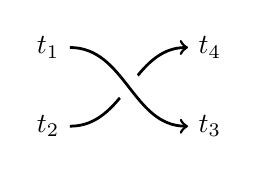
\begin{tikzpicture}[line width=1, baseline=10, scale=1]
    \draw[->] (0,0) node[left] {\(t_{2}\)} \br (1.5,1) node[right] {\(t_{4}\)};
    \draw[white, line width=10] (0,1) node[left] {} \br (1.5,0) node[right] {};
    \draw[->] (0,1) node[left] {\(t_{1}\)} \br (1.5,0) node[right] {\(t_{3}\)};
    %    \draw (.75,1) node[above] {\(\alpha_{\lN}\)};
    %    \draw (0,0.5) node {\(\alpha_{\lW}\)};
    %    \draw (.75,0) node[below] {\(\alpha_{\lS}\)};
    %    \draw (1.5,0.5) node {\(\alpha_{\lE}\)};
  \end{tikzpicture}
  \to
  \frac{1}{\nr}
  \crossingfunction{+}{\mu}{t_{1}, t_{2}, t_{3}, t_{4}}
  \\
  \label{eq:crossing negative}
  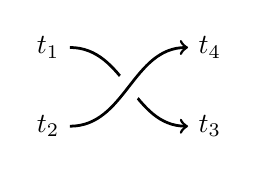
\begin{tikzpicture}[line width=1, baseline=10, scale=1]
    \draw[->] (0,1) node[left] {\(t_{1}\)} \br (1.5,0) node[right] {\(t_{3}\)};
    \draw[white, line width=10] (0,0) node[left] {} \br (1.5,1) node[right] {};
    \draw[->] (0,0) node[left] {\(t_{2}\)} \br (1.5,1) node[right] {\(t_{4}\)};
  \end{tikzpicture}
  \to
  \frac{1}{\nr}
  \crossingfunction{-}{\mu}{t_{1}, t_{2}, t_{3}, t_{4}}
\end{align}
(the factors of \(1/\nr\) are convenient when discussing asymptotics)
and assigning critical points shifts in the variables (which we could
also think of as \(\delta\) functions)
\begin{align}
  &
  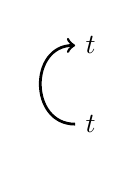
\begin{tikzpicture}[line width=1, baseline=10, scale=1]
    \draw[->, looseness = 1.5] (0,0) node[right] {\(t\)} to [out
    =180, in=180] (0,1) node[right] {\(t\)};
  \end{tikzpicture}
  &
  &
  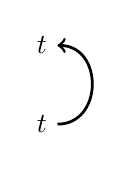
\begin{tikzpicture}[line width=1, baseline=10, scale=1]
    \draw[->, looseness = 1.5] (0,0) node[left] {\(t\)} to [out =0,
    in=0] (0,1) node[left] {\(t\)};
  \end{tikzpicture}
  &
  &
  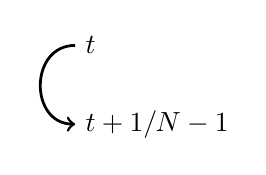
\begin{tikzpicture}[line width=1, baseline=10, scale=1]
    \draw[<-, looseness = 1.5] (0,0) node[right] {\(t + 1/\nr - 1\)}
    to [out =180, in=180] (0,1) node[right] {\(t\)};
  \end{tikzpicture}
  &
  &
  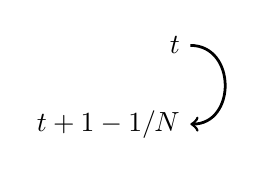
\begin{tikzpicture}[line width=1, baseline=10, scale=1]
    \draw[<-, looseness = 1.5] (0,0) node[left] {\(t + 1 - 1/\nr\)}
    to [out =0, in=0] (0,1) node[left] {\(t\)};
  \end{tikzpicture}
\end{align}

\begin{definition}
  We call \(\actq{D, \mu}{}\) the \defemph{action} of the diagram.
  Note that it depends on the diagram \(D\) and on \(\mu\) but
  \emph{not} on a choice of representation.
\end{definition}

\begin{example}
  \label{ex:figure eight}
  Below is an open diagram \(D\) of the figure eight knot:
  \begin{equation*}
    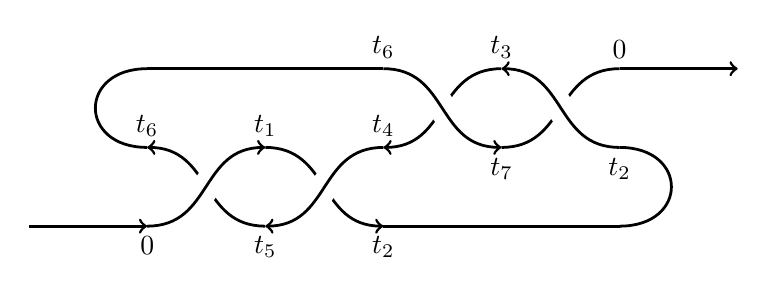
\begin{tikzpicture}[line width=1, scale=1, xscale=1.5]
      \draw[<-] (0,1) node[above] {\(t_{6}\)} \br (1,0) node[below] {\(t_{5}\)};
      \draw[white, line width=10] (0,0) node {} \br (1,1) node {};
      \draw[->] (0,0) node[below] {\(0\)} \br (1,1) node[above] {\(t_{1}\)};

      \draw[->] (1,1) node {} \br (2,0) node[below] {\(t_{2}\)};
      \draw[white, line width=10] (1,0) node {} \br (2,1) node {};
      \draw[<-] (1,0) node {} \br (2,1) node[above] {\(t_{4}\)};

      \draw[<-] (2,1) node {} \br (3,2) node {};
      \draw[white, line width=10] (2,2) node {} \br (3,1) node {};
      \draw[->] (2,2) node[above] {\(t_{6}\)} \br (3,1) node[below] {\(t_{7}\)};

      \draw[-] (3,1) node {} \br (4,2) node {};
      \draw[white, line width=10] (3,2) node {} \br (4,1) node {};
      \draw[<-] (3,2) node[above] {\(t_{3}\)} \br (4,1) node[below] {\(t_{2}\)};

      \draw (2,0) to (4,0) ;
      \draw[looseness = 1.5] (4,0) to [out =0, in=0] (4,1);

      \draw (0,2) to (2,2) ;
      \draw[looseness = 1.5] (0,1) to [out =180, in=180] (0,2);

      \draw[->] (-1,0) to (0,0);

      \draw[->] (4,2) node[above] {\(0\)} to (5,2);
    \end{tikzpicture}
  \end{equation*}
  Assigning variables to the segments as shown the action is
  \begin{align*}
    \actq{D, \mu}{t}
    &=
    \frac{1}{\nr}
    \crossingfunction{+}{\mu}{0, t_{5}, t_{1}, t_{6}}
    +
    \frac{1}{\nr}
    \crossingfunction{+}{\mu}{t_{4} + \tfrac{1}{\nr} - 1, t_{1}, t_{5}
    + \tfrac{1}{\nr} - 1, t_{2}}
    \\
    &\phantom{=}-
    \frac{1}{\nr}
    \crossingfunction{-}{\mu}{t_{3} + \tfrac{1}{\nr} - 1, t_{6}, t_{4}
    + \tfrac{1}{\nr} - 1, t_{7}}
    +
    \frac{1}{\nr}
    \crossingfunction{-}{\mu}{t_{7}, t_{2}, 0, t_{3}}
  \end{align*}
  The parameter shifts come from using critical points to rotate the
  crossings as in \cite[Figure 13]{McPhailSnyderVolume}.
\end{example}

Let \(\rho\) be a decorated representation of \(K\).
Choose an admissible, normalized shadow coloring \((\rho, u)\) of
\(D\) and a \defemph{log-meridian} \(\mu\), a logarithm of the
meridian eigenvalue \(m\) determined by the decoration.
(Recall that a normalized shadow coloring is one where the segment
parameter of the boundary segments is \(1\).)
Assume that the coloring is not pinched: if it is then \(\qinv{}\) is
still well-defined but we need to use a different expression for the
\(R\)-matrix coefficients.

Choose logarithms \(\beta_{i}\) of the segment parameters \(b_{i}\)
with \(e^{\tu \beta_{i}} = b_{i}\).
It is helpful to think of this choice as a vector \(\beta \in
\mathbb{C}^{E}\), where \(E\) is the set of internal segments.
We call \(\beta\) a \defemph{log-coloring}.
Since we are using a normalized coloring we can choose \(0\) as the
log-parameter of the boundary segments.
Re-writing \cite[Lemma 6.3]{McPhailSnyderVolume} in our normalizations gives

\begin{theorem}[\protect{\cite[Lemma 6.3]{McPhailSnyderVolume}}]
  \label{thm:state sum}
  The invariant \(\qinv{}\) defined in \cite{McPhailSnyderVolume} is
  given by the sum
  \begin{equation}
    \label{eq:state sum}
    \qinv{K, \rho, \mu}
    =
    \frac{1}{\nr^{|E|/2 + 1/2}}
    \sum_{n \in \nset{\nr}^{E}}
    e^{ \nr  \actq{D}{(\beta + n)/\nr} }
  \end{equation}
  where \(\nset{\nr} \defeq \set{0, 1, \dots, \nr -1}\).
  \( \qinv{K, \rho, \mu} \) is gauge-invariant, and in particular is
  independent of the choice of shadow coloring and log-coloring.
\end{theorem}

\begin{lemma}
  \label{thm:action lemmas}
  Let \(\beta\) be a log-coloring of a normalized, non-pinched shadow coloring.
  \begin{thmenum}
  \item
    \label{thm:action lemma:lattice periodic}
    \(t \mapsto \exp \nr \actq{D, \mu}{t}\) is a
    \(\mathbb{Z}^{E}\)-periodic function on the lattice
    \(
      \frac{\beta}{\nr} + \frac{1}{\nr}\mathbb{Z}^{E}
      .
    \)
  \item
    \label{thm:action lemma:no poles}
    If the shadow coloring avoids the unit circle, then none of the poles
    of the  function \(\mathbb{C}^{E} \to \mathbb{C}\) defined by
    \[
      t \mapsto \exp \nr \actq{D, \mu}{\beta/\nr + t}
    \]
    occur for \(t \in \mathbb{R}^{E}\).
    \qedhere
  \end{thmenum}

\end{lemma}

\begin{proof}
  \ref{thm:action lemma:lattice periodic}
  \Cref{eq:pfl recurrence} gives the quasi-periodicity relation
  \[
    e^{\pfl{\zeta/\nr + 1}}
    =
    \frac{
      e^{\pfl{\zeta/\nr}}
    }{
      (1 - e^{\tu (\zeta + 1)/\nr})
      \cdots
      (1 - e^{\tu (\zeta + \nr)/\nr})
    }
    =
    \frac{
      e^{\pfl{\zeta/\nr}}
    }{
      1 - e^{\tu \zeta}
    }
  \]
  so
  \begin{align*}
    \exp
    \crossingfunction{+}{\mu}{
      \frac{\beta_{1}}{\nr} + 1,
      \frac{\beta_{2}}{\nr},
      \frac{\beta_{1'}}{\nr},
      \frac{\beta_{2'}}{\nr}
    }
    &=
    \exp
    \crossingfunction{+}{\mu}{
      \frac{\beta_{1}}{\nr},
      \frac{\beta_{2}}{\nr},
      \frac{\beta_{1'}}{\nr},
      \frac{\beta_{2'}}{\nr}
    }
    \frac{
      (1- b_{2'}/b_{1})
    }{
      m(1- b_{2}/m b_{1})
    }
    \\
    &=
    a_{1}
    \exp
    \crossingfunction{+}{\mu}{
      \frac{\beta_{1}}{\nr},
      \frac{\beta_{2}}{\nr},
      \frac{\beta_{1'}}{\nr},
      \frac{\beta_{2'}}{\nr}
    }
  \end{align*}
  where \(a_{1}\) is the parameter assigned to the segment by
  \cref{eq:segment a vars}.
  Similarly
  \[
    \exp
    \crossingfunction{+}{\mu}{
      \frac{\beta_{1}}{\nr},
      \frac{\beta_{2}}{\nr},
      \frac{\beta_{1'}}{\nr} + 1,
      \frac{\beta_{2'}}{\nr}
    }
    =
    a_{1'}^{-1}
    \exp
    \crossingfunction{+}{\mu}{
      \frac{\beta_{1}}{\nr},
      \frac{\beta_{2}}{\nr},
      \frac{\beta_{1'}}{\nr},
      \frac{\beta_{2'}}{\nr}
    }
  \]
  and more generally the incoming segment variables have
  quasi-periodicity constant \(a_{i}\) and the outgoing have \(a_{i}^{-1}\).
  When the crossing functions \(\crossingfunction{\epsilon}{\mu}{}\)
  are assembled together into \(\actq{D,\mu}{}\) these factors
  cancel: the \(a_{i}\) match because the \(b_{i} = e^{\tu
  \beta_{i}}\) are a solution of the gluing equations.

  \ref{thm:action lemma:no poles}
  Recall that the zeros and poles of \(e^{\pfl{z}}\) all occur when
  \(z \in \frac{1}{\nr} \mathbb{Z}\).
  The arguments of the quantum dilogarithms \(\pfl{}\) in
  \cref{eq:crossing positive,eq:crossing negative}  are of the form
  \(\zeta/\nr + t_{i} -
  t_{j}\) with \(e^{\tu \zeta}\) the shape parameter of the relevant
  tetrahedron.
  Because \((\rho, u)\) avoids the unit circle \(\Im \zeta \ne 0\)
  for each tetrahedron so we do not encounter any singularities when
  \(t \in \mathbb{R}^{E}\).
\end{proof}

\subsection{State integrals}%
\label{sec:State integrals}

\begin{definition}
  \label{def:state integral}
  The \defemph{state integrals} associated to a log-coloring \(\beta\) are
  \begin{equation}
    \label{eq:state integral again}
    \stint{D, \mu, \beta}{k} \defeq
    \int_{[0,1]^{E}}
    \exp \nr \left( \actq{D, \mu}{t + \beta/\nr} - \tu k \cdot t \right)
    \dif t
  \end{equation}
  for each integer vector \(k \in \mathbb{Z}^{E}\).
\end{definition}

\begin{bigtheorem}
  \label{main result}
  Under the hypotheses above \(\qinv{}\) is given by the sum
  \begin{equation}
    \label{eq:state intgral sum}
    \qinv{K, \rho, \mu}
    =
    \nr^{|E|/2 - 1/2}
    \sum_{k \in \mathbb{Z}^{E}}
    \stint{D, \mu, \beta}{k}
  \end{equation}
  over all state integrals.
\end{bigtheorem}

\begin{proof}
  Define a function  \(F \colon \mathbb{R}^{E} \to \mathbb{C}\) by \(F(t)
  \defeq \exp (\nr \actq{D, \mu}{t + \beta/\nr})\).
  It restricts to a not-necessarily continuous, periodic function \(f
  \colon \mathbb{C}^{E}/\mathbb{Z}^{E} \to \mathbb{C}\).
  By \cref{thm:action lemmas}\ref{thm:action lemma:no poles} \(F\) is
  smooth and in particular
  \begin{equation}
    \label{eq:f-is-BV}
    \int_{[0,1]^{E}} \left| \frac{\partial F(t)}{ \partial t_{i}} \right| \dif t
    =
    \int_{\mathbb{C}^{E}/\mathbb{Z}^{E}} \left| \frac{\partial f(t)}{
    \partial t_{i}}
    \right| \dif t < \infty
    \text{ for all } i \in E.
  \end{equation}
  \(f\) has Fourier coefficients
  \(
    a_{k}
    \defeq
    \int_{[0,1]^{E}} f(t) e^{- \tu k \cdot t} \dif t
  \)
  and our claim is that
  \[
    \qinv{K, \rho, \mu}
    =
    \nr^{|E|/2 - 1/2}
    \sum_{k \in (\nr \mathbb{Z})^{E}}
    a_{k}
    .
  \]
  \Cref{eq:f-is-BV} says that \(f\) has bounded variation, so its Fourier series
  \(
    \sum_{k \in \mathbb{Z}^{E}} a_{k} e^{\tu k \cdot t}
  \)
  converges everywhere and converges to \(f(t)\) when \(t\) is a
  point of continuity for \(f\).
  By \cref{thm:action lemmas}\ref{thm:action lemma:lattice periodic}
  \(f\) is continuous on the lattice
  \(\left(\frac{1}{\nr}\mathbb{Z}\right)^{E}\), so when \(n \in \mathbb{Z}^{E}\)
  \[
    f(n/\nr)
    =
    \sum_{k \in \mathbb{Z}^{E}} a_{k} e^{\tu k \cdot n/\nr}.
  \]
  Plugging this into the state sum \eqref{eq:state sum} gives
  \[
    \qinv{K, \rho, \mu}
    =
    \frac{
      1
    }{
      \nr^{|E|/2 + 1/2}
    }
    \sum_{n \in [\nr]^{E}}
    f(n/\nr)
    =
    \frac{
      1
    }{
      \nr^{|E|/2 + 1/2}
    }
    \sum_{k \in \mathbb{Z}^{E}}
    a_{k}
    \sum_{n \in [\nr]^{E}}
    e^{\tu k \cdot n/\nr}
  \]
  As
  \(
    \sum_{n \in [\nr]^{E}}
    e^{\tu k \cdot n/\nr}
  \)
  is \(\nr^{|E|}\) if every component of \(k\) is divisible by
  \(\nr\) and \(0\) otherwise we conclude
  \[
    \qinv{K, \rho, \mu}
    =
    \nr^{|E|/2 - 1/2}
    \sum_{k \in (\nr \mathbb{Z})^{E}} a_{k}
    .
    \qedhere
  \]
\end{proof}

\section{Formal asymptotics}%
\label{sec:Formal asymptotics}

We conclude by formally studying the large \(\nr\) asymptotics of the
state integrals and discussing barriers to rigorously establishing them.

\subsection{Classical dilogarithms}%
\label{sec:Classical dilogarithms}

The computation of Chern-Simons invariants is closely related to a
special function called the \defemph{dilogarithm} defined by
\[
  \operatorname{Li}_{2}(z)
  \defeq
  - \int_{0}^{z} \frac{\log(1 - t)}{t} \, d t
\]
We refer to \textcite{Zagier2007} for more information on the dilogarithm.
It has a branch point at \(1\) and crossing the branch cut picks up a
\(\log(z)\) term, which itself has a branch point at \(0\).
Analytic continuation of \(e^{\operatorname{Li}_{2}(z)}\) leads to
the flattenings of \citeauthor{Neumann2004} \cite{Neumann2004}.
To avoid dealing with these in full generality, write \(X = (-\infty,
0] \cup [1, \infty)\) and consider \cite[Chapter 4]{Murakami2018} the
holomorphic function \(\dll{} \colon \mathbb{C} \setminus X \to
\mathbb{C}\) defined by
\begin{equation}
  \dll{\zeta}
  \defeq
  \begin{cases}
    \displaystyle
    \frac{
      \operatorname{Li}_{2}(e^{\tu \zeta})
    }{
      \tu
    }
    &
    \Im \zeta > 0
    \\
    \displaystyle
    -
    \frac{
      \operatorname{Li}_{2}(e^{-\tu \zeta})
    }{
      \tu
    }
    - \pi \ii \zeta(\zeta -1)
    - \frac{\pi \ii}{6}
    &
    \Im \zeta < 0
  \end{cases}
\end{equation}

\begin{lemma}
  \label{thm:dilog lemma}
  For fixed \(\zeta \in \mathbb{C} \setminus X \),
  \[
    \exp \frac{ \mathrm{d} \dll{\zeta}}{\mathrm{d} \zeta}
    =
    \frac{
      1
    }{
      1 - e^{\tu \zeta}
    }
  \]
  and
  \[
    e^{\pfl{\zeta}}
    =
    \exp\leftfun[
      \frac{
        \dll{\zeta + 1/2\nr}
      }{\nr}
      +
      \bigoh(\nr^{-1})
    \rightfun]
    \qedhere
  \]
\end{lemma}

\begin{proof}
  The first claim is an elementary computation.
  In the notation of \textcite{Murakami2018} we have \(
  e^{\pfl{\zeta}} = \psi_{\nr}(\zeta + 1/2\nr) \) so the second claim
  follows from \cite[eq.\ (4.3)]{Murakami2018}.
\end{proof}

\subsection{The classical action}%
\label{sec:The classical action}

Here we define an action \(\act{D}{}\) corresponding to the \(\nr \to
\infty\) limit of \(\actq{D}{}\).
Set
\begin{equation}
  \label{eq:crossing log}
  \begin{aligned}
    \crossingfunctionclass{+}{t_{1}, t_{2}, t_{3}, t_{4}}
    &\defeq
    \dll{t_{4} - t_{1}}
    +
    \dll{t_{2} - t_{3}}
    \\
    &\phantom{\defeq}
    -
    \dll{t_{2} - t_{1}  + 1 }
    -
    \dll{t_{4} - t_{3} }
    \\
    &\phantom{\defeq}
    - \tu(t_{2} - t_{1})
    \\
    \crossingfunctionclass{-}{t_{1}, t_{2}, t_{3}, t_{4}}
    &\defeq
    -
    \dll{t_{1} - t_{4} + 1}
    -
    \dll{t_{3} - t_{2} + 1}
    \\
    &\phantom{\defeq}
    +
    \dll{t_{1} - t_{2}}
    +
    \dll{t_{3} - t_{4} + 1}
    \\
    &\phantom{\defeq}
    + \tu(t_{2} - t_{1})
  \end{aligned}
\end{equation}
Assign complex variables \(t_{i}\) to the segments as before and
construct a function \(\act{D}{t}\) by taking a sum over crossing functions
\begin{align}
  \label{eq:crossing positive class}
  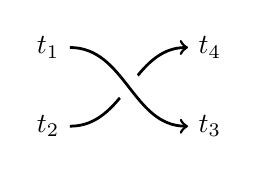
\begin{tikzpicture}[line width=1, baseline=10, scale=1]
    \draw[->] (0,0) node[left] {\(t_{2}\)} \br (1.5,1) node[right] {\(t_{4}\)};
    \draw[white, line width=10] (0,1) node[left] {} \br (1.5,0) node[right] {};
    \draw[->] (0,1) node[left] {\(t_{1}\)} \br (1.5,0) node[right] {\(t_{3}\)};
    %    \draw (.75,1) node[above] {\(\alpha_{\lN}\)};
    %    \draw (0,0.5) node {\(\alpha_{\lW}\)};
    %    \draw (.75,0) node[below] {\(\alpha_{\lS}\)};
    %    \draw (1.5,0.5) node {\(\alpha_{\lE}\)};
  \end{tikzpicture}
  \to
  \crossingfunctionclass{+}{t_{1}, t_{2}, t_{3}, t_{4}}
  \\
  \label{eq:crossing negative class}
  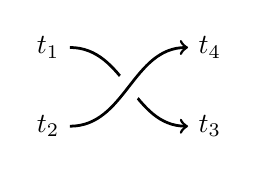
\begin{tikzpicture}[line width=1, baseline=10, scale=1]
    \draw[->] (0,1) node[left] {\(t_{1}\)} \br (1.5,0) node[right] {\(t_{3}\)};
    \draw[white, line width=10] (0,0) node[left] {} \br (1.5,1) node[right] {};
    \draw[->] (0,0) node[left] {\(t_{2}\)} \br (1.5,1) node[right] {\(t_{4}\)};
  \end{tikzpicture}
  \to
  \crossingfunctionclass{-}{t_{1}, t_{2}, t_{3}, t_{4}}
\end{align}
and assigning critical points shifts in the variables (which we could
also think of as \(\delta\) functions)
\begin{align}
  &
  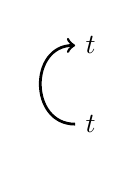
\begin{tikzpicture}[line width=1, baseline=10, scale=1]
    \draw[->, looseness = 1.5] (0,0) node[right] {\(t\)} to [out
    =180, in=180] (0,1) node[right] {\(t\)};
  \end{tikzpicture}
  &
  &
  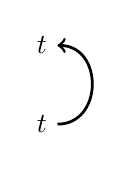
\begin{tikzpicture}[line width=1, baseline=10, scale=1]
    \draw[->, looseness = 1.5] (0,0) node[left] {\(t\)} to [out =0,
    in=0] (0,1) node[left] {\(t\)};
  \end{tikzpicture}
  &
  &
  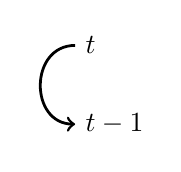
\begin{tikzpicture}[line width=1, baseline=10, scale=1]
    \draw[<-, looseness = 1.5] (0,0) node[right] {\(t - 1\)} to [out
    =180, in=180] (0,1) node[right] {\(t\)};
  \end{tikzpicture}
  &
  &
  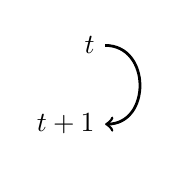
\begin{tikzpicture}[line width=1, baseline=10, scale=1]
    \draw[<-, looseness = 1.5] (0,0) node[left] {\(t + 1\)} to [out
    =0, in=0] (0,1) node[left] {\(t\)};
  \end{tikzpicture}
\end{align}

\begin{definition}
  The construction above defines the \defemph{classical action} as a
  holomorphic function
  \[
    \act{D}{} \colon \Omega_{D} \to \mathbb{C}
  \]
  where
  \[
    \Omega_{D} =
    \set{
      t \in \mathbb{C}^{E}
      \given
      t_{i} - t_{j} \not \in X
      \text{ whenever \(i,j\) meet at a corner of \(D\)}
    }
  \]
\end{definition}

The classical action is a variant of Yokota's \defemph{potential
function} introduced in \cite{arXiv:math/0009165} and used throughout
the Volume Conjecture literature.
We prefer to call it an \emph{action} to match the language used in
physics, since it is essentially the Chern-Simons action if we view
\(\Omega_{D}\) as parametrizing flat \(\mathfrak{sl}_{2}\)
connections on the knot complement.
Our action includes parameter shifts that appear to be related to the
normalization terms \(\Omega_{1}, \Omega_{2}\) studied by
\citeauthor{zbMATH06433029} \cite{zbMATH06433029}.

\begin{definition}
  A \defemph{generalized critical point} \(\gamma \in
  \mathbb{C}^{E}\) of the classical action is one where
  \[
    \exp
    \left.
    \frac{
      \partial \act{D}{}
    }{
      \partial t_{i}
    }
    \right|_{\gamma}
    =
    1
    \text{ for all } i \in E.
  \]
  or equivalently, a point for which there is a \defemph{flattening
  vector} \(k \in \mathbb{Z}^{E}\) with
  \[
    \left.
    \frac{
      \partial \act{D}{}
    }{
      \partial t_{i}
    }
    \right|_{\gamma}
    =
    \tu
    k_{i}
    \text{ for all } i \in E.
  \]
\end{definition}

\begin{proposition}
  \label{thm:crit points are reps}
  Let \(D\) be a diagram of a knot \(K\).
  Generalized critical points of \(\act{D}{}\) are in bijection with
  normalized non-pinched shadow colorings \((\rho,u)\) of \(D\) with
  meridian eigenvalue \(1\).
  If \(\gamma\) is the critical point corresponding to \((\rho, u)\),
  then its critical value is the \(\slg\) Chern-Simons invariant of
  \(\rho\) (which is independent of \(u\)).
  In the notation of \cite{McPhailSnyderVolume},
  \[
    \exp \act{D}{\gamma} = \mathcal{I}^{\psi}(K, \rho, u).\qedhere
  \]
\end{proposition}

\begin{proof}
  \Cref{thm:dilog lemma} shows that generalized critical points are
  equivalent to the segment equations for \(m = 1\), so we can apply
  \cref{thm:segment solutions are reps}.
  The second claim was worked out in detail by
  \citeauthor{zbMATH06370282} \cite{zbMATH06370282}.
  We explain the idea in our notation.
  In \cite{McPhailSnyderVolume} the Chern-Simons invariant
  \(\log \mathcal{I}^{\psi}\) is defined by taking a sum of
  contributions over crossings.
  However, instead of using the crossing functions \eqref{eq:crossing log}
  defined in terms of \(\dll{}\) \cite{McPhailSnyderVolume} uses
  lifted dilogarithms
  \[
    \lambda(\zeta)
    =
    \dll{\zeta} + \zeta \log(1 - e^{\tu \zeta})
  \]
  In general the extra terms \(\zeta \log(1 - e^{\tu \zeta})\) are
  nontrivial: they correspond to the gluing equations.
  At a critical point \(\gamma\) these are satisfied and the extra
  terms vanish modulo \(\mathbb{Z}\).
\end{proof}

\begin{remark}
  \label{rem:flattening vector}
  \textcite{Neumann2004} gave an algebraic method to compute the
  \(\slg\) Chern-Simons invariant of a triangulated manifold.
  The hyperbolic structure on \(M\) is encoded using a solution of
  Thurston's gluing equations as usual, but his method requires an
  additional choice of combinatorial data called a \defemph{flattening}.
  This is a coherent choice of logarithms of the shape parameters
  satisfying a logarithmic form of the gluing equations.
  For an octahedral decomposition the only nontrivial flattening
  equations come from the segment equations and are of the form
  \[
    \pm \mu + \log(1 - z_{j}) -  \log(1 - z_{j'})
    =
    \pm \mu + \log(1 - z_{l}) -  \log(1 - z_{l'})
    + k_{i}
  \]
  for an integer \(k_{i}\) at each segment.
  These are precisely the integers appearing in the flattening vector above.
\end{remark}

\subsection{Asymptotics}%
\label{sec:Asymptotics}

It is immediate from \cref{thm:dilog lemma} that \(\actq{D}{}\)
converges pointwise on \(\Omega_{D}\) to \(\act{D}{}\) as \(\nr \to
\infty\), which suggests we can approximate the state integrals
\(\stint{D, \mu, \beta}{k}\) of \eqref{eq:state integral again} by
using a saddle-point approximation.
\citeauthor{zbMATH06684922} gives a detailed explanation of the
saddle point approximation in the context of the Volume Conjecture in
\cite[Section 3]{zbMATH06684922}, which we summarize here.

Let \(f\) be holomorphic on some domain in  \(\mathbb{C}^{\ell}\)
containing an isolated critical point \(\gamma\).
A contour \(\Gamma \colon [-1,1]^{\ell} \to \mathbb{C}^{\ell}\) with
\(\Gamma(0) = \gamma\) passes through \(\gamma\) in \defemph{saddle
point position} if \(\Re f(\Gamma(t)) < \Re f(\gamma) \) except for
when \(t = 0\) and it satisfies an additional orientation condition.%
\note{
  For example, when \(\ell = 1\) the orientation condition says that
  \(\Gamma\) should go from one side of the mountain pass to the
  other, not double back.
}
The saddle point approximation says that
\[
  \int_{\Gamma} e^{\nr f(t)} \dif t
  =
  \nr^{-\ell/2}
  e^{\nr f(\gamma)}
  [ \tau + \bigoh(\nr^{-1}) ]
\]
for a constant \(\tau\) related to the determinant of the Hessian of
\(f\) at \(\gamma\).
It can be refined to include higher-order terms in the exponent whose
coefficients are related to derivatives of \(f\).
The idea is that near the critical point we can approximate \(e^{\nr
f}\) by a Gaussian.

We can apply this approximation to study the asymptotics of
\(\qinv{K, \rho, u}\) for \(K\) a hyperbolic knot.
Suppose there is some diagram \(D\) where \(\rho\) is not pinched;
as discussed in \cref{sec:Gauge transformations and admissibility} we
can think of this as a nondegeneracy condition on \(\rho\).
If we could show that \cref{step 2} holds then we could replace the
state integrals of \cref{eq:state integral again} with modified integrals
\[
  \stintadj{D}{k} \defeq
  \int_{\Gamma}
  \exp \nr \left( \act{D}{t} - \tu k \cdot t \right)
  \dif t
\]
for some other contour \(\Gamma\).
The dependence on the initial representation \(\rho\) drops out
because \(\beta/\nr \to 0\); this is one explanation for why the
growth rate in \eqref{eq:asymptotics sign positive} is independent of \(\rho\).
Changing the contour \(\Gamma\) is plausible because \(\act{D}{}\) is
a holomorphic function and we can use Stokes' Theorem (i.e.\ a
higher-dimensional Cauchy theorem) but there are other issues
discussed in \cref{sec:Barriers to Step 2}.

For now, suppose that it is valid to write
\begin{equation}
  \qinv{K, \rho, \mu}
  =
  \nr^{|E|/2 - 1/2}
  \sum_{k \in \mathbb{Z}^{E}}
  \stintadj{D}{k}
  +
  \bigoh(e^{\nr(\Re \varsigma_{K} - \delta)})
\end{equation}
for some \(\delta > 0\).
Since we assumed \(\rho\) was not pinched the complete hyperbolic
structure \(\rho_{\hyp}\) is also not pinched.
By \cref{thm:crit points are reps} there is a generalized critical
point \(\gamma\) of \(\act{D}{}\) with flattening vector \(k_{0}\)
corresponding to some normalized shadow coloring of \(\rho_{\hyp}\)
avoiding the unit circle.

We know that \(\act{D}{\gamma} = \varsigma_{K} \) is the \(\slg\)
Chern-Simons invariant of \(\rho_{\hyp}\) normalized as in
\cref{eq:asymptotics sign positive} and that \(\Re \varsigma_{K}\) is
maximal among all generalized critical points.
Suppose that \(\Gamma\) passes through \(\gamma\) in saddle point
position (which is not quite right: see below).
Then the saddle point approximation gives
\[
  \nr^{|E|/2 - 1/2}
  \stintadj{D}{k_{0}}
  =
  \tau
  \nr^{-1/2}
  e^{\nr \varsigma_{K} + \bigoh(\nr^{-1})}
\]
because \(\Gamma\) is an \(|E|\)-dimensional contour.
The terms of the sum with \(k \ne k_{0}\) do not contribute at
highest order to the asymptotics because the saddle point
approximation also requires the imaginary part of the derivative of
\(\act{D}{}\) to vanish: if it does not the growth is suppressed by
rapid oscillations in the phase of the integrand.
The sum over \(k\) in \eqref{eq:state intgral sum} naturally captures
the extra choice of flattening used in the computation of \(\varsigma_{K}\).

As noted above this analysis is incorrect.
The problem is that \(\gamma\) is \emph{never} an isolated critical
point because of gauge symmetry: the gauge transformations of
\cref{def:gauge transformation} show that a given representation
\(\rho\) corresponds to a manifold of complex dimension \(3\) lying in the
space \(\mathbb{C}^{E}\) of segment parameters.
If we restrict to normalized shadow colorings we fix one degree of
freedom, so \(\act{D}{}\) is \emph{constant} in two complex, hence four real
coordinate directions near \(\gamma\). This recovers an overall power
of \(\nr^{2}\), giving

\begin{conjecture}
  \label{our volume conjecture}
  Let \(K\) be a hyperbolic knot.
  Suppose that \(\rho\) is a decorated representation of \(D\) that
  is geometrically nondegenerate in the sense that \(\rho\) is
  non-pinched for some open diagram \(D\) of \(K\).
  Then for some choices of log-meridian \(\mu\) (see
  \cref{sec:Barriers to Step 2}) there is a constant \(\tau\) so that
  \begin{equation*}
    \qinv{K, \rho, \mu}
    =
    \nr^{3/2}
    e^{\nr \varsigma_{K} }
    [\tau + \bigoh(\nr^{-1}) ]
    \qedhere
  \end{equation*}
\end{conjecture}
Similar conjectures were made by  \citeauthor{zbMATH05624995}
\cite{zbMATH05624995}.

\subsection{Barriers to moving the contour}%
\label{sec:Barriers to Step 2}

\begin{figure}
  \centering
  \begin{tikzpicture}[line width=1]
    \draw (-2,0) to (2,0);
    \draw (0,-0.5) to (0,1);
    \draw[line width = 2, color=slred] (-2, 0) node[below] {\(X\)} to (0,0);
    \draw[line width = 2, color=slred] (1, 0) to (2, 0);
    \draw[->] (0,0) to (1.5, 1) node[above] {\(\zeta\)};
    \draw[color=slblue] (1.5-1,1) to (2.5, 1) node[right] {\(\zeta + [-1,1]\)};
    \draw[color=slblue] (.75-1,.5) to (1.75,.5) node[right]
    {\(\zeta/2 + [-1,1]\)};
  \end{tikzpicture}
  \caption{
    The arguments of the dilogarithms in the state integrals \(
    \stint{D, \mu, \beta}{k} \) are of the form \(\zeta/\nr + t_{i} -
    t_{j}\) with \(t_{i}, t_{j} \in [0,1]\).
    As \(\nr \to \infty\) the segments over which they vary approach
    the singular region \(X = (-\infty, 0] \cup [1, \infty)\).
  }
  \label{fig:approach singularities}
\end{figure}

Establishing the volume asymptotics of \cref{our volume conjecture}
requires replacing our original state integrals
\begin{equation*}
  \stint{D, \mu, \beta}{k} \defeq
  \int_{[0,1]^{E}}
  \exp \nr \left( \actq{D, \mu}{t + \beta/\nr} - \tu k \cdot t \right)
  \dif t
\end{equation*}
with shifted ones
\[
  \stintadj{D}{k} \defeq
  \int_{\Gamma}
  \exp \nr \left( \act{D}{t} - \tu k \cdot t \right)
  \dif t.
\]
This is \cref{step 2} for \(\qinv{}\).
The idea is to use Stokes' Theorem to shift the initial contour
\([0,1]^{E}\) to some new contour \(\Gamma\) in saddle position for
the correct critical point.
The obvious problem is that Stokes' Theorem can move only the
interior of the contour, not the boundary.%
\note{%
  If the integrand were periodic the boundary terms would cancel but
  this only holds on a lattice in \(\mathbb{C}^{E}\) as in
  \cref{thm:action lemmas}\ref{thm:action lemma:lattice periodic}.
}
This is a serious issue.
As shown in \cref{fig:approach singularities} the arguments of the
quantum dilogarithms in the action in the original state integral
approach the real axis as \(\nr \to \infty\).
Unfortunately the real axis is precisely where the problems are: as
\(\nr \to \infty\) the singularities of \(e^{\pm \pfl{}}\) become
dense in \(X\).
Near this region \(\actq{D, \mu}{}\)  can fail to uniformly converge
to \(\act{D}{}\), which is related to the fact that the branch points
of the dilogarithm lie there.
While the interior of the contour can be moved away the remaining
boundary will still approach the singular region.
Understanding why the remaining boundary terms cancel or do not
contribute is a hard analytic problem.
There may be subtleties here that obstruct \cref{our volume
conjecture} for certain \((\rho, \mu)\).

One case where this occurs is already known.
When \(\rho\) is boundary-parabolic experimental evidence
\cite[Remark 6.2]{McPhailSnyderVolume} suggests \(\qinv{K, \rho,
\mu}\) vanishes unless  \(2\mu \equiv -1 \pmod {\nr \mathbb{Z}}\).
This suggests there can be nontrivial cancellations in the sum
\eqref{eq:state intgral sum} and/or indicate other barriers to moving
the contour.
Examining these issues may shed light on why it sometimes \emph{is}
possible to move the contour and prove asymptotic growth.

\printbibliography

\end{document}

